% Allgemeine Probleme (Hard- und Software)

\chapter{Probleme}
\label{sec:probleme}
\section{Docker}
\label{subsec:probleme_docker}
\initials{LG}
%TODO wording?
Am Laptop von Herr Gastgeber war es am Beginn des Schuljahres nicht möglich,
jegliche Geräte im Netzwerk der HTL zu erreichen.
%
Grund dafür war eine Software namens Docker,
welche außerhalb dieses Projekts zur Containerisierung von anderen Anwendungen dient.
%
Docker war standardmäßig so konfiguriert,
dass es containerspezifische Subnets im IPv4-Adressbereich \allowbreak\texttt{172.117.0.0/16} erstellt.
%
Diese Subnets hatten dann am Laptop eine höhere Priorität als das Schulnetzwerk,
was dafür sorgte,
dass das weltweite Internet noch erreichbar war, 
nicht aber das lokale Schulnetzwerk.
%
Um Docker einen anderen IP-Adressbereich zuzuweisen,
wurde der Docker-Daemon mithilfe der Datei \texttt{/etc/docker/daemon.json}
wie in Listing \ref{lst:docker_address_pools} konfiguriert.
\begin{lstlisting}[language=json,gobble=4,
    label=lst:docker_address_pools,caption=Konfiguration für den Docker-Daemon]
    {
          "default-address-pools":
          [
            {"base":"10.10.0.0/16","size":24}
          ]
    }
\end{lstlisting}

\section{Modifikationen am Tumbller}
\label{subsec:problem_tumbbler_mods}
\initials{LG}
%TODO kein "wir"
Als wir das Projekt geplant haben,
war die Idee,
einfach ein fertiges Kit ein bisschen zu modifizieren,
fast schon zu schön um wahr zu sein.
%
Und das war es dann auch.
%
Bei den Hardware-Modifikationen am Tumbller (siehe Kapitel \ref{subsec:elegoo_tumbller}) gab es zwei relativ große Probleme:

\subsection{Falsche Betriebsspannungen}
\label{subsec:problem_betriebsspannungen}
\initials{LG}
Beim Austausch des mitgelieferten Arduino Nano mit einem ESP32 im Nano-Format haben wir einen wichtigen Faktor übersehen:
%
Der Arduino Nano hat eine Betriebsspannung von 5V,
während der ESP32 mit 3.3V arbeitet.
%
Glücklicherweise funktionieren die meisten Komponenten des Elegoo Tumbllers auch mit 3.3V.
%
Die einzigen Bauteile,
welche eine höhere Spannung benötigen,
sind die auf der Platine angelöteten farbigen Leuchtdioden.
%
Um nicht das ganze Projekt von Grund auf neu aufbauen zu müssen,
haben wir uns entschieden,
dieses kleine optische Detail fürs Erste auszulassen.
%
%TODO schaltplan
In der originalen Beschaltung (siehe Abbildung \ref{fig:elegoo_tumbller_original_circuit})
wurde das Bluetooth-Modul mithilfe des Spannungswandlers \texttt{U3} mit 3.3V versorgt.
%
Diesen Spannungswandler haben wir ausgebaut und mittels einer Lötbrücke $V_{in}$ mit $V_{out}$ verbunden.
Allerdings erwies sich das Bluetooth Modul später als problematisch (siehe Abschnitt \ref{subsec:problem_bluetooth_serial}),
weshalb die Überbrückung eigentlich nicht notwendig ist.
\\\\
Außerdem war es beim Guide-Roboter aufgrund des Wechsels auf 3.3V nicht mehr möglich,
den LiDAR-Sensor direkt mit dem Spannungswandler des Mikrocontroller-Boards zu versorgen.
%
Deshalb haben wir für den Guide einen zusätzlichen Step-Down-Konverter eingebaut,
welcher die Versorgungsspannung des Akkus auf 5V für den LiDAR herunterregelt.
\section{Blockierte UART-Schnittstelle}
\label{subsec:problem_bluetooth_serial}
\initials{LG}
Als das Problem der inkompatiblen Spannungen gelöst,
und die erste Version des Programmes zum Testen der einzelnen Komponenten geschrieben war,
%TODO Formulierung: "großes Problem" hab ich schon vorher verwendet
sind wir auch schon auf das nächste nennenswerte Problem gestoßen:
%
Das externe Bluetooth-Modul,
was bereits auf der Platine verlötet war,
belegt die UART-Schnittstelle des eingebauten ESP32.
%
Das führte dazu, dass der ESP32 nur neu programmiert werden konnte,
wenn das ESP32-Devboard aus dem Roboter ausgebaut war.
%
Außerdem wurde dadurch das Debuggen mittels UART über USB unmöglich gemacht.
\\
Da wir die Roboter über WLAN steuern,
und der ESP32 auch ohne externe Erweiterungen bereits sowohl über WLAN- als auch Bluetooth-Kapazitäten verfügt,
haben wir entschlossen,
die mitgelieferte Platine weiter zu modifizieren,
indem wir das Bluetooth-Modul entfernen.
%
Außerdem haben wir den Transistor \texttt{Q1} und den Spannungsteiler,
welcher aus \texttt{R9} und \texttt{R10} besteht entfernt,
um sicherzustellen, das die UART-Verbindung keinesfalls beeinflusst wird
(siehe Original-Schaltplan in Abbildung \ref{fig:elegoo_tumbller_original_circuit}).
%TODO Bilder und Erläuterung zu Entfernen des Bluetooth Moduls


\section{Nicht identische Pinbelegung}
% TODO muss überarbeitet werden?
\label{subsec:arduino_to_esp32}
\initials{JS}
Der Wechsel zum ESP32 Nano lief nicht reibungslos wie erhofft da,
obwohl der ESP von Arduino das "gleiche Gehäuse" verwendet 
es jedoch zu einigen Unterschieden in den Pins kommt. 

% TODO änder die pins aufs wichtige
\begin{figure}[H]
    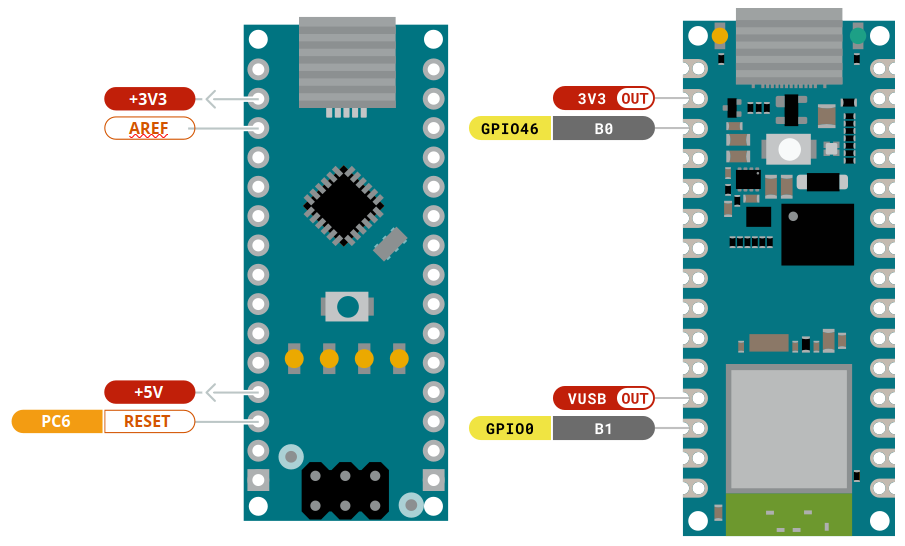
\includegraphics[width=\textwidth, center]{img/nano-differences-m.png}
    \caption{Hervorgehobene Pinbelegung zwischen Arduino und ESP32 nano}
    \label{fig:nano_boards}
\end{figure}

Zwischen den Boards herrschen für dieses Projekt am wesentlichen diese Unterschiede.
\begin{itemize}
    \item Pin 3 von \texttt{AREF} zu \texttt{GPIO46} und \texttt{Boot0}.
    \item Pin 12 von \texttt{+5V} zu \texttt{VUSB} oder \texttt{VBUS}.
    \item Pin 13 von \texttt{RESET} zu \texttt{GPIO0} und \texttt{Boot1}.
\end{itemize}

Der Pin 3 von \texttt{AREF} ist unproblematisch aufgrund dessen dass,
es zu einem ungenutzten I/O Interface führt und somit keinem weiteren Besorgen.

Bei Pin 12 muss etwas Achtung gegeben werden, weil der \texttt{VBUS} im Vergleich zu \texttt{+5V} als
direkte Führung von der Versorgung aus der USB Schnittstelle bedacht wurde und 
dadurch nicht weiter geregelt wird vom Board. Deswegen wird empfohlen den VBUS 
nicht mit anderen Pins am Nano kurz zuschließen, jedoch wenn der ESP32 über den VIN Pin versorgt ist, 
wird der Pin deaktiviert und sollte keine 5V von der USB Schnittstelle liefern können. 
% Weiteres verhalten darüber hinaus ist nicht dokumentiert.
% Mehr dazu und der anderen Betriebsspannung ist in Abschnitt \ref{subsec:problem_betriebsspannungen} zu finden.

Pin 13 sollte keine Probleme machen da es zu einem offenen Schalter geht,
der ursprünglich den \texttt{RESET} Pin betätigt hätte und sonst offen liegt. 
Beim ESP32 würde der Schalter dafür sorgen das zum Boot Mode gewechselt werden kann, 
oder gewöhnliche Operationen mit \texttt{GPIO0}. 
Jedoch kam es zu Störungen an diesem Pin trotz internen Pull-up-Widerstand, 
wodurch wir den Pin entfernt haben mehr dazu siehe Abschnitt \ref{subsec:gestoert_boot}.


\section{Gestörter Boot Prozess} \label{subsec:gestoert_boot}
\initials{JS}
In unseren nächsten Test nachdem wir das Bluetooth-Modul entfernt haben 
und erfolgreich code laden konnten, verweigerte der ESP wieder den Programmierungprozess.
% TODO Bild und erkläarung zu fehlersuche
TODO

Dieser Pin 13 welcher ursprünglich als Reset agierte war nun verantwortlich für GPIO0. 
Jedoch sollte dies keine Probleme bescheren da der Pin offen liegt, weil der Schalter ein Schließer ist,
und nach ESP ein internen Pull-up Widerstand am GPIO0 liegt, kamen es trotzdem zu Störungen.
% https://docs.espressif.com/projects/esptool/en/latest/esp32/advanced-topics/boot-mode-selection.html#gpio0
Daraufhin haben wir den Pin entfernt, um die Störungen komplett zu vermeiden. 
Dies hatte die Folge das bei den Boards wo, die Bluetooth-Module noch nicht entfernt wurden,
jetzt auch neu programmiert werden konnte, ohne jegliche Modifikationen zum Bluetooth-Modul.
